%%% Preamble
\documentclass{report}

\usepackage[utf8]{inputenc}
\usepackage[T1]{fontenc}
\usepackage{fourier}
\usepackage[french]{babel}
\usepackage[protrusion=true,expansion=true]{microtype}	
\usepackage{amsmath,amsfonts,amsthm} % Math packages
\usepackage[pdftex]{graphicx}	
\usepackage{url}
\usepackage{pdfpages}
\usepackage{todonotes}
\usepackage[a4paper, body={16cm,26cm}]{geometry}
\usepackage{float}
\usepackage{framed}
\usepackage[toc,page]{appendix} 
\usepackage{multicol}
\usepackage{colortbl}
\usepackage{epstopdf}
\usepackage{adjustbox}

%%% Custom sectioning
\usepackage{sectsty}
\allsectionsfont{  \normalfont\scshape}
%\allsectionsfont{\centering \normalfont\scshape}

%%% Custom headers/footers (fancyhdr package)
\usepackage{fancyhdr}
\pagestyle{fancyplain}
\fancyhead{}								% No page header
\fancyfoot[L]{}							% Empty 
\fancyfoot[C]{}							% Empty
\fancyfoot[R]{\thepage}					% Pagenumbering
\renewcommand{\headrulewidth}{0pt}		% Remove header underlines
\renewcommand{\footrulewidth}{0pt}		% Remove footer underlines
\setlength{\headheight}{13.6pt}


%%% Equation and float numbering
\numberwithin{equation}{section}		% Equationnumbering: section.eq#
\numberwithin{figure}{section}		% Figurenumbering: section.fig#
\numberwithin{table}{section}		% Tablenumbering: section.tab#


%%% Define new commands
\newcommand{\horrule}[1]{\rule{\linewidth}{#1}} 	% Horizontal rule
\renewcommand{\bf}[1]{\textbf{#1}}
\renewcommand{\it}[1]{\textit{#1}}
\newcommand{\bfit}[1]{\textbf{\textit{#1}}}
\renewcommand{\sc}[1]{\textsc{#1}}

\newcommand{\Todo}[1]{\todo[inline]{#1}}
\renewcommand{\thesection}{\thepart .\arabic{section}}

\usepackage{tocloft}
\cftsetindents{chapter}{0em}{1em}
\cftsetindents{section}{1.5em}{2.5em}
\makeatletter
\def\l@figure{\@dottedtocline{1}{1.5em}{4em}}
\makeatother

\usepackage{bookmark}
%\usepackage[hidelinks]{hyperref}
\usepackage{cases}
\usepackage{color}
\usepackage{xcolor}
\usepackage{relsize}
\usepackage{caption}
\colorlet{shadecolor}{black!10}

\delimitershortfall-1sp
\newcommand\abs[1]{\left|#1\right|}


\usepackage{tikz, pgfplots}


%}}}
%{{{ --- pgfplots ---------------------

%{{{ Colors

% TolColors from http://www.r-bloggers.com/the-paul-tol-21-color-salute/
\definecolor{TolColor1}{HTML}{332288}   % dark purple
\definecolor{TolColor2}{HTML}{6699CC}   % dark blue
\definecolor{TolColor3}{HTML}{88CCEE}   % light blue
\definecolor{TolColor4}{HTML}{44AA99}   % light green
\definecolor{TolColor5}{HTML}{117733}   % dark green
\definecolor{TolColor6}{HTML}{999933}   % dark brown
\definecolor{TolColor7}{HTML}{DDCC77}   % light brown
\definecolor{TolColor8}{HTML}{661100}   % dark red
\definecolor{TolColor9}{HTML}{CC6677}   % light red
\definecolor{TolColor10}{HTML}{AA4466}  % light pink
\definecolor{TolColor11}{HTML}{882255}  % dark pink
\definecolor{TolColor12}{HTML}{AA4499}  % light purple

%}}}
%{{{ Color cycles

\pgfplotscreateplotcyclelist{mbarplot cycle}{%
  {draw=TolColor2, fill=TolColor2!70},
  {draw=TolColor7, fill=TolColor7!70},
  {draw=TolColor4, fill=TolColor4!70},
  {draw=TolColor11, fill=TolColor11!70},
  {draw=TolColor1, fill=TolColor1!70},
  {draw=TolColor8, fill=TolColor8!70},
  {draw=TolColor6, fill=TolColor6!70},
  {draw=TolColor9, fill=TolColor9!70},
  {draw=TolColor10, fill=TolColor10!70},
  {draw=TolColor12, fill=TolColor12!70},
  {draw=TolColor3, fill=TolColor3!70},
  {draw=TolColor5, fill=TolColor5!70},
}

\pgfplotscreateplotcyclelist{mlineplot cycle}{%
  {TolColor2, mark=*, mark size=1.5pt},
  {TolColor7, mark=square*, mark size=1.3pt},
  {TolColor4, mark=triangle*, mark size=1.5pt},
  {TolColor6, mark=diamond*, mark size=1.5pt},
}


\pgfplotsset{
  compat=1.9,
  mbaseplot/.style={
    legend style={
      draw=none,
      fill=none,
      cells={anchor=west},
    },
    x tick label style={
      font=\footnotesize
    },
    y tick label style={
      font=\footnotesize
    },
    legend style={
      font=\footnotesize
    },
    major grid style={
      dotted,
    },
    axis x line*=bottom,
  },
  mlineplot/.style={
    mbaseplot,
    xmajorgrids=true,
    ymajorgrids=true,
    major grid style={dotted},
    axis x line=bottom,
    axis y line=left,
    legend style={
      cells={anchor=west},
      draw=none
    },
    cycle list name=mlineplot cycle,
  },
  mbarplot base/.style={
    mbaseplot,
    bar width=6pt,
    axis y line*=none,
  },
  mbarplot/.style={
    mbarplot base,
    ybar,
    xmajorgrids=false,
    ymajorgrids=true,
    area legend,
    legend image code/.code={%
      \draw[#1] (0cm,-0.1cm) rectangle (0.15cm,0.1cm);
    },
    cycle list name=mbarplot cycle,
  },
  horizontal mbarplot/.style={
    mbarplot base,
    xmajorgrids=true,
    ymajorgrids=false,
    xbar stacked,
    area legend,
    legend image code/.code={%
      \draw[#1] (0cm,-0.1cm) rectangle (0.15cm,0.1cm);
    },
    cycle list name=mbarplot cycle,
  },
  disable thousands separator/.style={
    /pgf/number format/.cd,
      1000 sep={}
  },
}


%%  ========   IMPORTANT ========
%% Spécifier ici les variables pour le document
\newcommand{\mainTitle}{\'Etude préalable - SPIE}
\newcommand{\secondTitle}{Plan Assurance Qualité}
\newcommand{\documentRef}{PAQ/4401/1}

%%% Begin document
\begin{document}
%----------------------------------------------------------------------------------------
%	PACKAGES
%----------------------------------------------------------------------------------------

\documentclass[12pt]{article}
\usepackage[a4paper]{geometry}
\geometry{verbose,tmargin=1in,bmargin=0in,lmargin=1in,rmargin=1in}
\usepackage[utf8]{inputenc}
\usepackage[francais]{babel}
\usepackage[T1]{fontenc}

\usepackage{graphicx}
\begin{document}

\begin{titlepage}

\newcommand{\HRule}{\rule{\linewidth}{0.5mm}} % horizontal lines

\center % Center everything
 
%----------------------------------------------------------------------------------------
%	HEADING SECTIONS
%----------------------------------------------------------------------------------------

\vspace*{1cm}

\textsc{\LARGE INSA de LYON}\\[1.5cm] 
\textsc{\Large D\'epartement Informatique}\\[0.5cm] 
\textsc{\large Projet Longue Durée}\\[0.5cm] % 

%----------------------------------------------------------------------------------------
%	TITLE SECTION
%----------------------------------------------------------------------------------------

\HRule \\[0.4cm]
{ \huge \bfseries Compte Rendu}\\[0.1cm]
{\large \bfseries - Gestion des contacts commerciaux d'une banque -} 
\HRule \\[1.5cm]
 
%----------------------------------------------------------------------------------------
%	DATE SECTION
%----------------------------------------------------------------------------------------

{\large \today}\\[2cm] % 
 
%----------------------------------------------------------------------------------------
%	AUTHOR SECTION
%----------------------------------------------------------------------------------------

\begin{minipage}{0.4\textwidth}
\begin{center} \large
\emph{Auteurs} \\
Lisa \textsc{Courant} \\
Estelle \textsc{Lepeigneux} \\
Pierre \textsc{Jarsaillon} \\
Hugues \textsc{Verlin} \\
\end{center}
\end{minipage}
~
\begin{minipage}{0.4\textwidth}
\begin{center} \large
\emph{Chef de projet} \\
Paul \textsc{Dautry}
\end{center}
\begin{center} \large
\emph{Responsable Qualité} \\
Antoine \textsc{Chabert}
\end{center}
\end{minipage}\\[5cm]

H4401\\[2cm]

%----------------------------------------------------------------------------------------
%	LOGO SECTION
%----------------------------------------------------------------------------------------

\includegraphics[scale=0.3]{figures/logo.png}
%----------------------------------------------------------------------------------------

\vfill % Fill the rest of the page with whitespace

\end{titlepage}
\end{document}


\listoftodos
\newpage
\addcontentsline{toc}{part}{Tables des matières}
\tableofcontents
\addcontentsline{toc}{part}{Listes des figures}
\listoffigures
\addcontentsline{toc}{part}{Listes des tableaux}
\listoftables
\newpage
%\addcontentsline{toc}{part}{Introduction}
%\part{Introduction}
%\setcounter{section}{0}
%\section{Présentation du contenu du rapport}

%\include{file} % Inclusion du fichier file.tex présent dans le même répertoire

% ------------------ Première partie : contexte -----------------
\part{Objectifs}
\setcounter{section}{0}

\section{Généralités}

La recherche et l’élaboration d’une solution pour l’entreprise vise à livrer un ensemble de livrables spécifiant le résultat proposé. C’est dans le cadre de la réalisation de ces livrables qu’intervient le Plan d'Assurance Qualité (PAQ) afin de certifier l’état des documents produits. Ce document permet notamment de décrire les processus pour créer, sauvegarder, archiver et envoyer un livrable.

\section{Évolution du PAQ}

Le plan d’assurance qualité a été défini en début de projet et ne peut pas faire l’énumération ou l’explication de toutes les démarches de qualité. C’est pourquoi ce document est amené à évoluer pendant le déroulement du projet notamment pour les cas suivants : \\

\begin{itemize}
    \item[\textbullet] Défaut, incohérence ou imprécision dans le PAQ.
    \item[\textbullet] Après réflexion, une meilleure solution a été trouvée et devrait être appliquée.
    \item[\textbullet] Une bonne pratique a été identifié, il faut la formaliser et l’ajouter. \\
\end{itemize}

Tout changement doit avoir l’accord du responsable qualité et du chef de projet avant son intégration au PAQ. \\

Chaque modification du PAQ devra être notifiée à l’ensemble de l’équipe projet et chaque membre devra en prendre connaissance et s’informer en cas de questionnement ou d’incompréhension.
    
\section{En cas de non-respect du PAQ}
    
Dans les cas de non-respect du PAQ, la personne en charge du document à livrer sera directement informé par le responsable qualité ou le chef de projet afin de corriger les défauts. En aucun cas le document sera validé si le plan qualité n’est pas entièrement appliqué. \\

Un non-respect du plan qualité peut avoir de grandes conséquences. En effet, un retard plus ou moins important en découlera, avec une livraison dans les temps plus complexe et risquée. Éventuellement un dépassement des temps prévus et donc des coûts. C’est pourquoi, les membres de l’équipe doivent bien être conscients des risques afin de suivre à la lettre les règles du PAQ.
    
\section{Procédure de dérogation}

La rigueur du PAQ est là pour garantir une harmonie des livrables et un bon déroulement de projet. Cependant dans certains cas très précis et justifiés, une dérogation pourra être délivrée suite à l’accord du chef de projet et du responsable qualité. Si ce n’est pas le cas, la procédure de non-respect du PAQ sera appliquée.

% ------------------ Seconde partie : livrables -----------------
\part{Domaine d’application}
\setcounter{section}{0}
Ce présent document s’applique à l’ensemble des livrables conçus dans le cadre du projet, c’est-à-dire à l’ensemble de la documentation produite par les membres de l’équipe. Ces derniers doivent donc prendre connaissance du présent document, tandis que son application se doit d’être contrôlée par le responsable qualité. Lorsque le plan d’assurance qualité est amené à être modifié pour les raisons évoquées dans les paragraphes précédents, le responsable qualité a pour charge de communiquer à l’équipe les changements apportés, afin de veiller à ce que tous les membres soient au fait des nouvelles pratiques à appliquer. \\

Ainsi, tout document produit au sein de ce projet est soumis au procédé ci-dessous, consistant à appliquer le plan d’assurance qualité afin de produire un premier document par la maîtrise d’ouvrage. Le responsable qualité peut alors être amené à réaliser un rappel de ce plan d’assurance qualité auprès de la maîtrise d’ouvrage si certains concepts, procédés ou contraintes n’ont pas été respectés, afin d’obtenir un document normalisé pouvant être soumis à validation. Ce déroulement s’inscrit dans un cycle de vie des documents plus vaste et décrit dans la partie suivante.

\begin{figure}[H]
    \centering
    \label{fig-objec}
    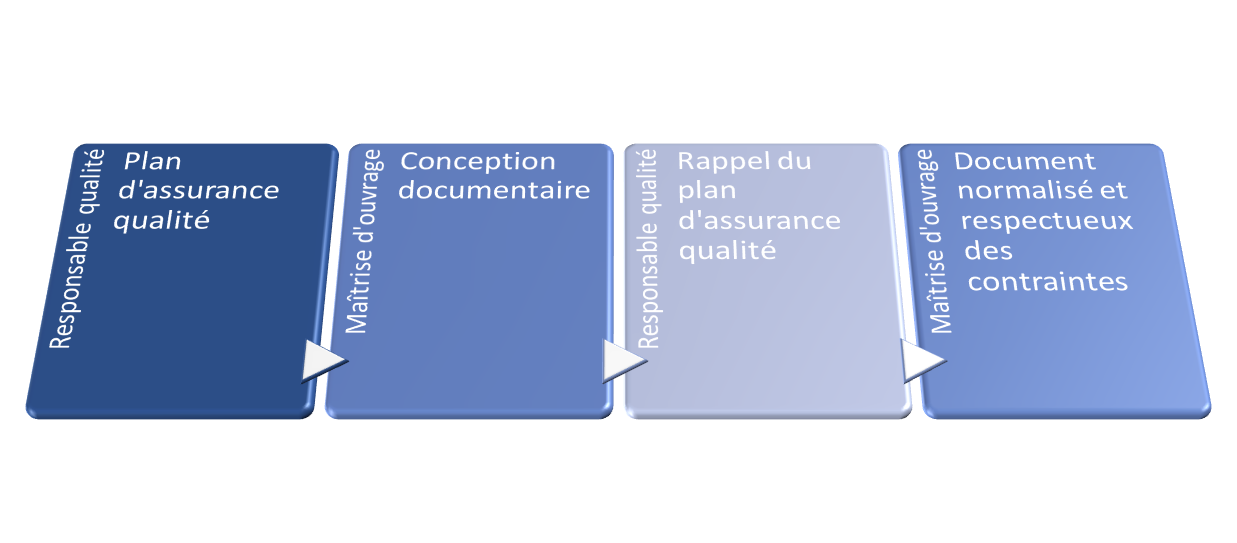
\includegraphics[scale=0.5]{figures/applic_paq.png}
    \caption{Application du plan d’assurance qualité lors de la conception d’un document}
\end{figure}
% ------------------ Troisième partie : méthodes et outils -----------------
\part{Gestion de la documentation}
\setcounter{section}{0}

\section{Stockage des documents}

Le projet comportant de nombreux livrables à portée interne comme externe, il est donc nécessaire de mettre en place une gestion de la documentation, simplifiant ainsi la gestion des livrables. Un espace de stockage est tout d’abord nécessaire afin de sauvegarder et d’archiver les différents documents produits par l’équipe de collaboration. Pour cela, l’outil Google Drive sera utilisé, donnant ainsi accès à tous les membres de l’équipe aux documents du projet. Afin de faciliter davantage l’organisation des documents, un dossier par phase (initialisation, expression du besoin…) sera créé sur cet espace de stockage, en addition du dossier spécifique aux tâches de gestion de projet.
 
\todo{Insérer le diagramme manquant ici...}

\section{Collaboration de la rédaction}

En combinaison avec l’espace de stockage Google Drive, l’outil Google Docs sera également utilisé pour créer et éditer les différents documents texte, tandis que l’outil Google Sheets sera utilisé pour les feuilles de calcul. Ces deux outils collaboratifs permettent de travailler à plusieurs sur les documents, tout en réalisant une gestion d’historique. Ainsi, des vérifications à intervalle régulier seront effectuées sur les documents, ces derniers étant facilement accessibles.
 
\section{Mise en forme et stockage final}

Lorsqu’un document est en version finale (se référer au paragraphe « Cycle de vie des documents » pour plus d’information), celui-ci est pris en charge par la qualité, qui débute le processus de recette. Lors de cette étape, le responsable qualité transforme le document Google Docs (ou Google Sheets, le cas échéant) afin d’obtenir un document au format LaTeX, garantissant ainsi l’uniformité des livrables. Le document au format LaTeX est ensuite transformé en fichier au format PDF, représentant ainsi la version de recette. Ces documents au format LaTeX et PDF sont ensuite archivés sur un dépôt Git, permettant ainsi de prévoir une gestion des versions de recette tout en proposant une sauvegarde distante.
 
Enfin, la livraison des documents finaux, au format PDF, sera effectuée via la plateforme Moodle, qui comporte les différents dépôts de données associés aux livrables attendus par le client.

Ainsi, les changements de format des différents documents produits au sein du projet peuvent être résumés à travers le schéma ci-dessous, de la création collaborative à l’archivage et la livraison de la version transformée au format PDF.

\todo{Insérer le diagramme manquant ici...}
% ------------------ Quatrième partie : activites, taches et planning -----------------
\part{Cycle de vie des documents}
\setcounter{section}{0}

\section{Généralités}

Afin de garantir l’homogénéité et la qualité des livrables, il est nécessaire de définir un cycle de vie des documents. Ainsi, chaque document devant être produit au cours du projet devra respecter les différentes étapes dudit cycle de vie. Lorsqu’un nouveau document entre en production au sein du projet, celui-ci sera soumis à deux phases principales. La première correspond à la procédure interne de vérification, réalisée par l’équipe, de façon collaborative, et visant à vérifier le contenu du document. La seconde phase correspond à la procédure de recette client, réalisée par le responsable qualité et par le chef de projet, permettant ainsi de valider le document en vérifiant notamment la mise en forme. L’enchaînement global des étapes au sein des phases est représenté dans le schéma ci-dessous, tandis que le détail de chaque phase est explicité à travers les sous-paragraphes ci-après.

\todo{Insérer le diagramme manquant ici...}

\section{Procédure interne de vérification}
    
Lorsqu’un nouveau document doit être établi, celui-ci entre directement dans la phase de procédure interne de vérification. Le document est alors créé grâce à l’outil Google Docs évoqué précédemment, en mode partagé afin que tous les collaborateurs disposent d’un accès à celui-ci. Afin de disposer d’un suivi avancé sur le document, un cartouche est directement apposé sur la première page de ce nouveau document. Le format du cartouche est alors le suivant : \\

\todo{L'exemple de cartouche manquant ici...}

Après ajout de ce cartouche, le document passe alors dans l’étape de production-rédaction, où chaque collaborateur a la possibilité de modifier et améliorer le document, en fonction de ses compétences et expertises. Lorsqu’un nouveau collaborateur contribue à l’amélioration du document, celui-ci a l’obligation d’ajouter son nom sur le cartouche, à l’emplacement intitulé « Auteurs du document ». \\
 
Des vérifications sont également effectuées à intervalle régulier sur le document par les différents acteurs qui, après satisfaction, valident leur étape de production en signant le cartouche, à l’emplacement prévu, situé sous l’intitulé « Auteurs du document » et en informent le relecteur assigné du document. Ce dernier doit impérativement être extérieur à la réalisation du document, afin de garantir une impartialité d’opinion sur le contenu du document. \\
 
Ensuite, l’étape de vérification est effectuée dans un premier temps par le relecteur assigné, puis par le responsable qualité. Cela permet de confirmer le passage du document en phase de procédure de recette client si aucune remarque n’est à relever. A contrario, en présence d’erreurs ou d’incohérences, le document retourne à l’étape de production. Pour cela, une nouvelle ligne est ajoutée au cartouche, permettant ainsi de tracer les différents changements d’étape. \\
 
L’enchaînement des étapes de cette phase du cycle de vie des documents est représenté à travers le schéma ci-dessous, tandis que la phase suivante est décrite dans le paragraphe ci-après. \\

\todo{Insérer le diagramme manquant ici...}

\section{Procédure interne de validation}
    
Lorsqu’un document termine sa phase de procédure interne de vérification, celui-ci débute la phase de procédure de recette client. Cette phase consiste à transformer le document collaboratif, sans mise en forme initiale, en un document répondant aux critères de qualité et respectant un format défini, à l’aide du format LaTeX. Cette étape de transformation, ou recette, est réalisée par le responsable qualité, qui veille à respecter les standards définis au préalable, afin de garantir l’uniformité des livrables. Après réalisation de cette étape, le responsable qualité appose sa signature sur le cartouche, à l’emplacement situé sous l’intitulé « Responsable qualité ». \\
 
Le document débute alors la dernière étape de son cycle de vie, qui correspond à la validation. Cette étape permet de garantir une dernière fois la bonne mise en forme du document, tout en déclarant le document terminé après avoir réalisé une dernière relecture, empêchant ainsi toute retouche par la suite. Cette étape est réalisée conjointement par le responsable qualité et par le chef de projet. Le document devient alors un document livrable, au format PDF, pouvant être archivé et livré au client. \\
 
Le déroulement de cette phase de recette client est résumé à travers le schéma ci-dessous.

\todo{Insérer le diagramme manquant ici...}

\section{Procédure de recette externe}

Lorsqu’un document est considéré comme étant livrable, ce dernier doit être soumis au client. Afin d’attester ladite livraison à une date donnée, prouvant ainsi le respect des délais, un procès-verbal de livraison est édité. Ainsi, le chef de projet modifie le document type disponible en annexe XX, adaptant ce dernier au livrable devant être fourni au client. Les informations importantes à mentionner dans ces procès-verbaux de livraison sont les suivantes : \\

\begin{itemize}
    \item[\textbullet] Référence et intitulé du livrable
    \item[\textbullet] Récepteur du livrable : nom et signature
    \item[\textbullet] Émetteur du livrable : nom et signature
    \item[\textbullet] Date de la livraison \\
\end{itemize}

Ces procès-verbaux de livraison sont produits en double exemplaire, permettant ainsi à l’émetteur et au récepteur du livrable de posséder une attestation de remise. Les deux partis s’engagent ainsi, par leur signature, à clôturer le cycle de vie du document livré, ce dernier ne pouvant être retouché par la suite.

% ------------------ Cinquième partie : organisation equipe -----------------
\part{Contraintes de validation }
\setcounter{section}{0}
\section{Contraintes générales}

Afin qu’un document puisse être considéré comme conforme puis, in fine, valide, il est nécessaire de définir, pour chaque livrable, les différentes contraintes à respecter. Ces contraintes s’appliquant à la fois sur la structure et le contenu des livrables. Nous pouvons définir pour ces derniers leur squelette, à travers la définition de leur plan.

\section{Squelettes documentaires}

\bf{Livrable DI/4401/1 - Dossier d’initialisation} \\

\begin{enumerate}
    \item Objet et contexte du projet
    \item Livrables
    \item Méthode et outils choisis
    \item Identification des activités et des tâches
    \item Planning
    \item Organisation de l’équipe
    \item Procédures validation/recette
    \item Gestion des risques \\
\end{enumerate}

\bf{Livrable PAQ/4401/2 - Dossier qualité} \\

\begin{enumerate}
    \item Objectifs
    \item Domaine d'application
    \item Gestion de la documentation
    \item Cycle de vie des documents
    \item Contrainte de validation 
    \item Outils utilisés
    \item Conclusion \\
\end{enumerate}

\bf{Livrable EE/4401/3 - Étude de l’existant} \\

\begin{enumerate}
    \item Contexte de l'étude
    \item Périmètre métier et fonctionnel
    \item Description du système d'information organisé
        \begin{enumerate}
            \item Les processus métier/fonctionnels
            \item La description des données
            \item La structure organisationnelle
        \end{enumerate}
    \item Description du système informatique
        \begin{enumerate}
            \item Les applications
            \item L'architecture technique \\
        \end{enumerate}
\end{enumerate}

\bf{Livrable BM/4401/4 - Benchmarking} \\

\begin{enumerate}
    \item Synthèse de scénarios de processus
    \item Progiciels généralistes ou spécialisés et principales fonctionnalités
    \item Analyse de l'adéquation globale des solutions et référentiels présentés \\
\end{enumerate}

\bf{Livrable SSC/4401/5 - Spécification du SI cible} \\

\begin{enumerate}
    \item Nouveaux modèles
    \item Modèles de l'existant modifiés
    \item Règles de gestion principales
    \item Axes d'amélioration \\
\end{enumerate}

\bf{Livrable SSP/4401/6 - Spécification d’une solution spécifique} \\

\begin{enumerate}
    \item Solution Informatique
        \begin{enumerate}
            \item Architecture applicative
                \begin{enumerate}
                    \item Liste des blocs applicatifs
                    \item Description des blocs : outils/service et données
                    \item Échange de données entre les blocs
                    \item Modèle d’architecture d’exécution
                    \item Schéma général
                \end{enumerate}
            \item Architecture technique
                \begin{enumerate}
                    \item Éléments actifs : réseau, serveurs, postes de travail
                    \item Architecture logicielle
                \end{enumerate}
        \end{enumerate}
    \item Solution organisationnelle \\
\end{enumerate}

\bf{Livrable SST/4401/7 - Spécification d’une solution standard} \\

\begin{enumerate}
    \item Introduction
    \item Vue globale 
    \item Vue organisationnelle 
    \item Vue informationnelle macro 
    \item Vue fonctionnelle
    \item Glossaire \\
\end{enumerate}

\bf{Livrable MCE/4401/8 - Modélisation et configuration d’une solution ERP} \\

\begin{enumerate}
    \item Introduction
    \item Vue globale de la chaîne de valeur SPIE
    \item Vue organisationnelle 
    \item Vue informationnelle 
    \item Vue fonctionnelle
    \item Glossaire  \\
\end{enumerate}

\bf{Livrable DC/4401/9 - Dossier de choix} \\

\begin{enumerate}
    \item Pour chaque solution
        \begin{enumerate}
            \item Rappel des fonctionnalités de la solution informatique et organisationnelle
            \item Chiffrages des coûts
            \item Retour sur investissement
            \item Évaluation des autres critères de comparaison
        \end{enumerate}
    \item Tableau comparatif et pondération
    \item Recommandations \\
\end{enumerate}
 
\bf{Livrable RDB/4401/10 - Restitution document bilan} \\

\begin{enumerate}
    \item Résumé des documents précédents
    \item Évolution du produit attendu
    \item Bilan des charges \\
\end{enumerate}

\bf{Livrable DB/4401/11 - Dossier bilan} \\

\begin{enumerate}
    \item Les phases du projet
        \begin{enumerate}
            \item Phase d’organisation du projet
            \item Phase d’expression des besoins
            \item Phase d’analyse de scénario
            \item Phase d’évaluation du projet
        \end{enumerate}
    \item Répartition de la charge de travail
    \item Suivi du moral et de la bonne humeur
    \item Suivi de la qualité
    \item Bilans personnels 
\end{enumerate}

\section{Identification des documents}

Les documents constituant les livrables sont tous identifiés par  une référence unique qui est construite de la manière suivante \it{$<$CodeTextuelDuLivrable$>$}/4401/\it{$<$NumeroDeVersionDuLivrable$>$}.

Le \it{$<$CodeTextuelDuLivrable$>$} est construit sur l'intitulé du livrable, généralement les initiales des mots constituant cet intitulé. 

Le \it{$<$NumeroDeVersionDuLivrable$>$} est quant à lui utilisé pour réaliser l'historique des révisions et permet au client de suivre les corrections apportées.

% ------------------ Sixième partie : procedures de validation et recette -----------------
\part{Outils utilisés}
\setcounter{section}{0}
\section{Gestion de projet}

Pour communiquer facilement dans l’équipe, nous utilisons un outil spécialisé dans le domaine, Slack. En effet, ce dernier permet de communiquer sur le projet, quelque soit la localisation des membres de l’équipe et quelque soit l’équipement technique de ces derniers. \\

Pour gérer l’avancement des différentes tâches et avoir une vision des responsabilités de chacun, nous utilisons l’outil Google Sheet, assimilable à un classeur Excel, qui permet également d’avoir des statistiques sur les temps passés, les avancements et les délais.

\section{Gestion des documents}

Comme indiqué précédemment, nous utilisons dans un premier temps un outil dédié au travail collaboratif pour éditer les documents, Google Docs. Puis, afin d’appliquer une mise en page identique à tous les documents, nous utilisons l’outil LaTeX à travers l’éditeur TeXMeX.

\section{Gestion des livrables}

Afin de gérer les différentes versions des livrables et les stocker facilement, nous utilisons à la fois Google Drive ainsi que l’outil spécialisé Git à travers un dépôt hébergé sur un serveur personnel.

\section{Gestion des diagrammes}

La gestion des diagrammes est réalisée à travers divers outils, en fonction du type de digramme à gérer. Concernant les diagrammes répondant de la méthode UML, l’outil PlantUML est utilisé, permettant ainsi d’uniformiser les différents diagrammes, grâce à une description textuelle de ces derniers. \\

Les digrammes ARIS sont réalisés grâce à l’outil spécialisé ARIS Architect, qui offre l’ensemble des méthodes et composants nécessaires à la réalisation des différents modèles.

\section{Gestion de données ERP}

Concernant la gestion des informations reliées aux ERP, l’outil spécialisé SAP est utilisé, mettant ainsi à disposition toutes les fonctionnalités nécessaires au projet, tout en profitant de l’expertise du responsable SAP de l’équipe projet.
% ------------------ Septième partie : livrables -----------------
\part{Conclusion}
\setcounter{section}{0}
\section{Conclusion}

Ce plan d’assurance qualité est certes un document ayant pour objectif d’assurer la qualité de l’ensemble des livrables produits durant un projet en garantissant une normalisation et une harmonisation des documents. Cependant, cela demande un engagement de la part du responsable qualité qui doit veiller à sa bonne application au sein du projet par les membres de l’équipe. \\

Les besoins du client SPIE sont également pris en compte dans le présent document. Ce document représente ainsi vis à vis du client un gage de qualité, illustrant l’engagement de l’équipe projet quant à l’aboutissement de celui-ci, tout en veillant à répondre aux besoins du client.  \\

S’inscrivant dans une politique d’amélioration continue, ce plan d’assurance qualité n’est pas immuable. Celui-ci est en effet ouvert aux rectifications jugées comme apportant une plus-value aux documents produits.

% ------------------ Annexe -----------------
\appendix
\chapter{Procès Verbal de Livraison}

\begin{table}[H]
    \centering
    \begin{tabular}{l}
        \multicolumn{1}{c}{
        \begin{tabular}[c]{@{}c@{}}
            \bf{Procès-verbal de livraison}\\ PV/4401/\it{$<$CodeTextuelEtNumeroDeVersionLivrable$>$}\end{tabular}} \\
        \begin{tabular}{@{}p{15cm}@{}}
            \\ Document remis : le document intitulé \it{$<$Intitulé livrable$>$}, référencé \it{$<$RéférenceDocument$>$} \\ \\ \it{$<$DestinataireDuLivrable$>$} reconnaît par le présent procès-verbal avoir reçu ce jour le \it{$<$99/99/9999$>$}, le livrable \it{$<$DescriptifDuLivrable$>$} remis, remis par l’hexanôme H4401 comme prévu dans le dossier d’initialisation (ref. DI/4401/1) rendu le 11/12/2015. Il s’engage ainsi à procéder à la clôture du livrable référencé \it{$<$RéférenceLivrable$>$}, se soustrayant ainsi à toute requête ultérieure de modification.
        \end{tabular} \\
    \end{tabular}
\end{table}
\begin{table}[H]
    \centering
    \begin{tabular}{ll}
        \multicolumn{1}{c}{\textbf{}}                                                                                                              & \multicolumn{1}{r}{
        \begin{tabular}[c]{@{}r@{}}
            Fait à Villeurbanne en deux exemplaires, \\ Le \it{$<$99/99/9999$>$}
        \end{tabular}} \\
        \begin{tabular}[c]{@{}l@{}}
            \\Pour l’hexanôme H4401, Pour \it{$<$DestinataireDuLivrable$>$} \\ \\ Le Chef de projet, \\ Monsieur Paul Dautry
        \end{tabular} \\                                                                                                               
    \end{tabular}
\end{table}



%%% End document
\end{document}
